
En este capítulo se explica la metodología CRISP-DM (Cross-Industry Standard Process for Data Mining), que se utiliza en el desarrollo del resto del proyecto para alcanzar los objetivos propuestos.

La adopción de metodologías estructuradas es fundamental en el desarrollo de proyectos informáticos, puesto que proporcionan un marco sistemático para garantizar la calidad, eficiencia y trazabilidad del proyecto. En particular, metodologías como CRISP-DM, permiten: alinear objetivos técnicos con necesidades de negocio,reducir riesgos mediante fases iterativas y documentadas, y facilitar la colaboración entre equipos multidisciplinares.

Según algunos estudios, los proyectos que utilizan metodologías estandarizadas incrementan un 35\% su probabilidad de éxito, frente a aproximaciones \textit{ad-hoc}, al minimizar desviaciones en costes y plazos \cite{chapman2000crisp}. En el ámbito de la ciberseguridad, donde los requisitos legales y técnicos son críticos, este enfoque metodológico resulta indispensable para asegurar soluciones robustas y auditables

\section{CRISP-DM}
La metodología CRISP-DM, es un marco de trabajo estandarizado para guiar proyectos de minería de datos y aprendizaje automático. Su estructura cíclica y flexible la hace aplicable en diversos dominios, desde marketing hasta ciberseguridad. Está compuesta por las siguientes fases:

\textbf{1. Comprensión del negocio:} La primera fase de CRISP-DM establece los cimientos estratégicos del proyecto mediante un proceso de alineación entre los objetivos técnicos y las necesidades organizacionales. Para lograr establecer los cimientos, se lleva a cabo un análisis exhaustivo del contexto empresarial para identificar los problemas clave que el proyecto debe abordar, así como las oportunidades de mejora que podrían aprovecharse. Se realiza un proceso de recopilación y documentación de requisitos que involucra a todas las partes interesadas relevantes. El resultado de esta fase es una definición precisa del alcance del proyecto, que incluye no solo los objetivos cuantificables sino también los criterios de éxito que permitirán evaluar el impacto real de la solución propuesta. Además, se establecen las limitaciones operativas y estratégicas que condicionarán el desarrollo del proyecto, asegurando que todas las fases posteriores se ejecuten dentro de un marco bien definido y alineado con las prioridades organizacionales.


\textbf{2. Comprensión de los datos:} Esta fase se centra en el análisis detallado de los datos disponibles para el proyecto, con el objetivo de evaluar su idoneidad y calidad para abordar los problemas identificados en la fase anterior. Este proceso implica un examen minucioso de las diversas fuentes de información, su estructura y sus características fundamentales. Durante esta etapa, se identifican y documentan aspectos críticos como la complejidad de los datos, la presencia de posibles sesgos y la representatividad de la información en relación con los objetivos del proyecto. La comprensión profunda de los datos permite anticipar desafíos potenciales y establecer estrategias adecuadas para su tratamiento en fases posteriores. Además, esta fase proporciona perspectivas que pueden influir en decisiones técnicas importantes, como la selección de algoritmos o el diseño de características. El resultado es un conocimiento del potencial y las limitaciones de los datos disponibles, que sirve como base para las transformaciones que se realizan en la siguiente fase.

\textbf{3. Preparación de los Datos:} Se trata de una fase crítica donde los datos brutos se transforman en un conjunto adecuado para modelado. Esta etapa implica una serie de operaciones fundamentales que garantizan la calidad y consistencia de los datos que alimentan a los modelos analíticos. Las actividades realizadas en esta fase son cruciales para el éxito del proyecto, ya que determinan en gran medida la capacidad de los algoritmos para extraer patrones significativos y generar resultados confiables. Se aplican técnicas especializadas para abordar problemas comunes en los datos, asegurando que la información sea representativa, completa y se encuentre adecuadamente estructurada para los análisis posteriores. Cualquier deficiencia en la preparación de los datos puede comprometer significativamente la efectividad de las siguientes fases. Al finalizar este proceso, se obtiene un conjunto de datos optimizado que conserva la esencia de la información original mientras elimina ruido y distorsiones que podrían afectar negativamente a los resultados del modelado.


\textbf{4. Modelado:} Constituye el núcleo técnico del proceso CRISP-DM, donde se desarrollan y evalúan los algoritmos diseñados para extraer conocimiento de los datos preparados. Esta etapa comienza con la selección cuidadosa de las técnicas de modelado más apropiadas para los objetivos específicos del proyecto y las características de los datos disponibles. Durante el proceso de modelado, se exploran diferentes enfoques algorítmicos, ajustando meticulosamente sus parámetros para optimizar su rendimiento. En esta fase se incluyen procesos de validación diseñados para garantizar que los modelos desarrollados sean robustos y generalizables, capaces de mantener su efectividad cuando se enfrenten a datos nuevos y no vistos previamente. El modelado es un proceso iterativo que puede requerir volver a fases anteriores para refinar la preparación de datos o incluso reconsiderar algunos aspectos del planteamiento inicial del problema. El resultado de esta fase es uno o varios modelos validados que cumplen con los criterios de calidad establecidos y están listos para su evaluación en el contexto de los objetivos empresariales definidos inicialmente.  

\textbf{5. Evaluación:} Esta fase representa un examen exhaustivo de los modelos desarrollados, contrastando su desempeño técnico con los objetivos empresariales establecidos en la primera fase del proyecto. Este proceso va más allá de las métricas estadísticas tradicionales para incorporar una valoración del impacto potencial de la solución propuesta. Durante la evaluación, se analiza minuciosamente la capacidad de los modelos para resolver el problema de negocio original, considerando tanto su precisión técnica como su aplicabilidad práctica en el contexto organizacional. Se identifican y documentan las limitaciones de los modelos, así como los posibles riesgos asociados a su implementación. Esta fase también incluye la validación de los resultados con las partes interesadas clave, asegurando que la solución cumpla con las expectativas y requisitos operativos. La evaluación termina con una decisión fundamentada sobre la idoneidad de los modelos para su implementación, junto con recomendaciones para su posible mejora o adaptación a escenarios futuros. También se valida su robustez en escenarios realistas.

\textbf{6. Despliegue:} Se trata de la fase final de CRISP-DM, esta se centra en la transición del modelo analítico desde un entorno de desarrollo a un sistema operativo donde pueda generar valor tangible para la organización. Este proceso implica una serie de actividades cuidadosamente planificadas que garantizan la integración efectiva de la solución en los procesos empresariales existentes. El despliegue incluye aspectos técnicos como la implementación de la infraestructura necesaria, el desarrollo de interfaces adecuadas y la creación de mecanismos de monitoreo continuo. También se ha de tener en cuenta la capacitación de los usuarios finales y la documentación exhaustiva de la solución, asegurando su adopción efectiva y su uso óptimo. La fase de despliegue también establece procesos para el mantenimiento y actualización periódica del modelo, puesto que las soluciones analíticas requieren evolución continua para mantener su relevancia y efectividad. Como en el resto de metodologçias, se implementan mecanismos para medir el impacto real de la solución una vez en producción, cerrando el ciclo al proporcionar retroalimentación valiosa que puede ser la base de futuros proyectos analíticos.

Como se ha explicado, CRISP-DM es una metodología iterativa, esto significa que los resultados de fases posteriores pueden revelar la necesidad de ajustes en etapas anteriores (como recolectar más datos o redefinir objetivos). Su enfoque estructurado minimiza riesgos y maximiza el valor entregado, siendo especialmente útil en proyectos complejos donde la alineación entre técnica y negocio es esencial.

\begin{figure}[htbp]
    \centering
    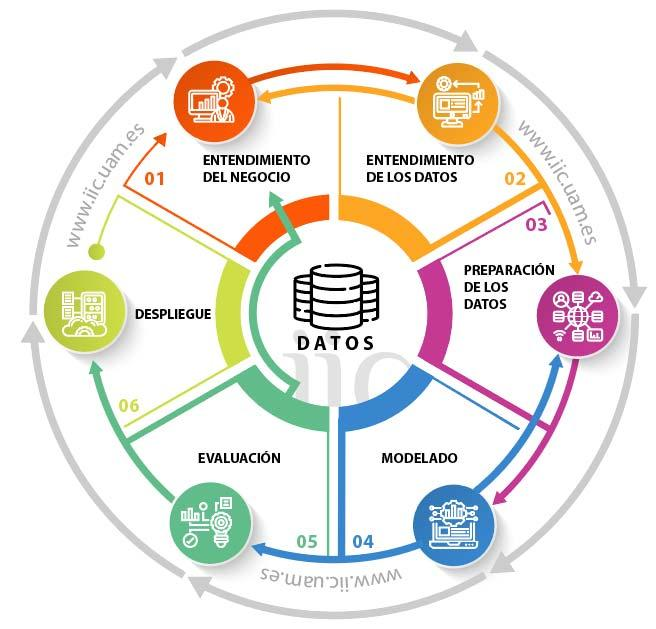
\includegraphics[width=0.8\textwidth]{./img/metodologia/crispdm.jpeg}
    \caption{Esquema del ciclo CRISP-DM estándar. \cite{haya_crisp_dm}}
    \label{fig:CRISP-DM}
\end{figure}